\documentclass{article}
\usepackage{algpseudocode}
\usepackage{amsfonts}
\usepackage{amsmath}
\usepackage{MnSymbol}
\usepackage[left=3cm, right=3cm, top=3cm]{geometry}
\usepackage{color}
\usepackage{tikz}

%Tikz settings for causal graphs
\usetikzlibrary{shapes,decorations,arrows,calc,arrows.meta,fit,positioning}
\tikzset{
    -Latex,auto,node distance =1 cm and 1 cm,semithick,
    state/.style ={ellipse, draw, minimum width = 0.7 cm},
    point/.style = {circle, draw, inner sep=0.04cm,fill,node contents={}},
    bidirected/.style={Latex-Latex,dashed},
    el/.style = {inner sep=2pt, align=left, sloped}
}

\renewcommand{\thesubsection}{\thesection.\alph{subsection}}

\title{HW2t}
\date{2018-10-12}
\author{Eric Boxer}

\begin{document}
\noindent Eric Boxer UNI ecb2198 Homework 2

\section{}
$X_1 \upmodels X_2 | X_3$ can be represented with any of the following graphs:

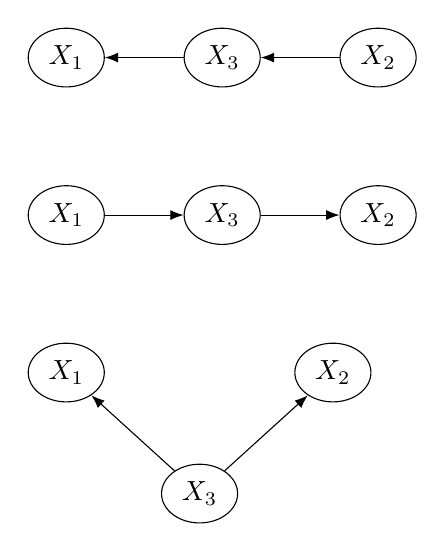
\begin{tikzpicture}
  \node[state] (x) at (0, 0) {$X_1$};

  \node[state] (y) [right =of x] {$X_3$};

  \node[state] (z) [right =of y] {$X_2$};

  \path (y) edge (x);

  \path (z) edge (y);

  \node[state] (x1) at (0, -2) {$X_1$};

  \node[state] (y1) [right =of x1] {$X_3$};

  \node[state] (z1) [right =of y1] {$X_2$};

  \path (x1) edge (y1);

  \path (y1) edge (z1);

  \node[state] (x2) at (0, -4) {$X_1$};

  \node[state] (y2) [below right =of x2] {$X_3$};

  \node[state] (z2) [above right =of y2] {$X_2$};

  \path (y2) edge (x2);

  \path (y2) edge (z2);
\end{tikzpicture}

\noindent Since $X3$ d-separates $X1$ and $X2 \implies X1 \upmodels X2 | X3$ and we know that the only conditional independence is between $X1, X2$
\section{}
(a) $Z = \emptyset$

\noindent Paths are: $X1 \rightarrow X2 \leftarrow X6 \rightarrow X7$ Blocked by collider $X2$

\noindent $X1 \rightarrow X2 \rightarrow X4 \rightarrow X5 \leftarrow X7$ Blocked by collider $X5$

\noindent $X1 \rightarrow X3 \rightarrow X4 \rightarrow X5 \leftarrow X7$ Blocked by collider $X5$

\noindent $X1 \rightarrow X3 \rightarrow X4 \leftarrow X2 \leftarrow X6 \rightarrow X7$ Blocked by collider $X4$

\noindent (b) $Z = \{X4, X6 \}$

\noindent Paths are: $X2 \rightarrow X4 \rightarrow X5$ Blocked by $X4 \in Z$

\noindent $X2 \leftarrow X1 \rightarrow X3 \rightarrow X4 \rightarrow X5$ Blocked by $X4 \in Z$

\noindent $X2 \leftarrow X6 \rightarrow X7 \rightarrow X5$ Blocked by $X6 \in Z$

\noindent (c) $Z = \{X2, X3, X6\} $

\noindent $X1 \rightarrow X3 \rightarrow X4 \rightarrow X5$ Blocked by $X3 \in Z$

\noindent $X1 \rightarrow X3 \rightarrow X4 \leftarrow X2 \leftarrow X6 \rightarrow X7 \rightarrow X5$ Blocked by $X3 \in Z$

\noindent $X1 \rightarrow X2 \rightarrow X4 \rightarrow X5$ Blocked by $X2 \in Z$

\noindent $X1 \rightarrow X2 \leftarrow X6 \rightarrow X7 \rightarrow X5$ Collider $X2$ is unblocked by including, but the path is blocked by $X6 \in Z$

\section{}
\noindent (a) $Z = \emptyset$ All paths enumerated above are blocked back-door paths so we do not need to condition on anything.

\noindent (b) $Z = \{X1, X6\}$ Of the paths above, the first is a direct causal path and must not be blocked. The other two are back-door paths and are blocked by $X1$ and $X6$, respectively.

\section{}
D-separation blocks every path between two nodes and is commutative. In other words, if $X$ is d-separated with $Y$ then $Y$ is d-separated with $X$, since every path from $X$ to $Y$ is a path from $Y$ to $X$ and vice-versa. In contrast, the back-door criterion leaves causal paths unblocked, see the difference in sets $Z$ that d-separate $X2$ and $X5$ from the set satisfying the BDC. The set satisfying the BDC does not d-separate the two nodes, because we have left the direct causal path unblocked. Also, the BDC for $X$ on $Y$ is not commutative. For example, the set $Z$ satisfying the BDC for $X2$ on $X5$ does not satisfy the BDC for $X5$ on $X2$ because it leaves back-door path $X5 \leftarrow X4 \leftarrow X2$ unblocked.

\section{}

(a)

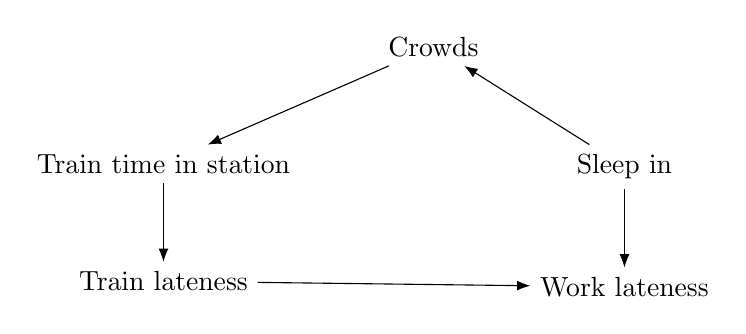
\begin{tikzpicture}
  \node (1) at (0, 0) {Crowds};
  \node (2) [below left =of 1] {Train time in station};
  \node (3) [below =of 2] {Train lateness};
  \node (4) [below right =of 1] {Sleep in};
  \node (5) [below =of 4] {Work lateness};

  \path (1) edge (2);
  \path (2) edge (3);
  \path (3) edge (5);
  \path (4) edge (1);
  \path (4) edge (5);
\end{tikzpicture}

\noindent (b)

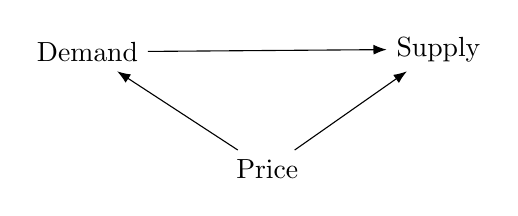
\begin{tikzpicture}
  \node (1) at (0, 0) {Demand};
  \node (2) [below right =of 1] {Price};
  \node (3) [above right =of 2] {Supply};

  \path (1) edge (3);
  \path (2) edge (1);
  \path (2) edge (3);
\end{tikzpicture}

\noindent Price has a causal effect on demand. Similarly, price has a causal effect on supply and as a result price creates a statistical dependence between demand and supply. Given some price $p$, an increase in demand will result in an accompanying increase in supply. Demand and supply are also indirectly correlated through collider supply.
\end{document}
